\chapter{The Responsible Human Being}

This chapter follows J. Krishnamurti's fourth San Diego conversation with Dr. Alan W. Anderson in the Krishnamurti Foundation Trust source material, curated for this course by LazyingArt LLC with Video2Book. The lecture is not a mathematical physics lecture, and there are no validated board images or visible equations for this chapter. Still, the conversation has a rigorous conceptual structure. We will use a little notation to keep the distinctions steady: responsibility as direction or as ground, action from formula or action now, choice from confusion or action from clarity, image as division, abstraction as escape from fact. These formulas are reading aids, not claims that Krishnamurti wrote equations on a board.

\section{Responsible For, Or Being Responsible}

Anderson opens by returning to the precise point where the previous conversation had stopped. The question is the distinction between being ``responsible for my action'' and simply being responsible. Krishnamurti does not treat this as a grammatical refinement. He makes it the hinge of the whole inquiry.

To be responsible for something already introduces a direction. It points toward a defined object, duty, institution, person, task, or field of action. The mind is then likely to carry an image of what action should be, and that image becomes a form of directed will. In the most compact notation,

\begin{equation}
\text{responsible for } X
\;\longrightarrow\;
\text{direction}+\text{directed will}.
\end{equation}

Being responsible has a different character. It is not responsibility in one particular direction. It includes education, politics, religion, business, conduct, the child, the neighbor, nature, and the whole movement of living, but it is not confined by any one of them. Krishnamurti calls it the ground in which action takes place.

\begin{equation}
\text{being responsible}
\;\longrightarrow\;
\text{total responsibility, not in a particular direction}.
\end{equation}

The first false map is therefore exposed at once. We usually imagine that responsibility becomes more exact when it is assigned to a definite object: my family, my job, my nation, my action. Krishnamurti reverses this. The object may already have narrowed the mind. It may already have turned responsibility into will operating along a track.

Anderson then brings in the continuous crisis they had been discussing. If crisis is not occasional but continuous, then the phrase ``my action'' can be misleading. It places action outside me, as though first there were an agent and then an action owned by that agent. Krishnamurti accepts Anderson's sharper formulation: I am my action. Responsibility is not a later moral attachment to action; it is the quality of action when the mind is not acting from a preconceived formula.

\begin{table}
\centering
\begin{tabular}{|p{0.43\linewidth}|p{0.43\linewidth}|}
\hline
\textbf{Responsible for} & \textbf{Being responsible} \\
\hline
Directed toward a particular object or field & Total, not confined to one direction \\
\hline
Carries the danger of will and preconceived action & Becomes the ground from which action takes place \\
\hline
May depend on a formula of what should be done & Requires seeing what is now \\
\hline
Can become responsibility to state, institution, role, or image & Expresses itself in the whole of life \\
\hline
\end{tabular}
\caption{A compact reconstruction of the opening distinction. No screenshot or board evidence is available for this lecture.}
\end{table}

\section{Action Now, Not Action From Formula}

Krishnamurti immediately tests the distinction in education. If one is totally responsible, what is one's responsibility toward children? Are they being educated to conform to the pattern society has established? Are they being trained into success, nationality, division, and therefore war? The question is not sentimental. It is a test of whether responsibility has escaped the narrow channel of ``responsible for'' and entered the whole field of life.

The local obstacle is then stated directly: if I say I am responsible for my action, what is that action based on? If it is based on a formula handed down by society, state, ideology, scripture, tradition, or collective habit, can it be responsible action?

\subsection{Question \& Answer}

\paragraph{Question.}
How can action be responsible if it is the result of a formula handed down from the past?

\paragraph{Answer.}
It cannot be responsible in Krishnamurti's sense, because the formula has already decided the movement. The action may be called duty, obedience, morality, patriotism, religion, or good citizenship, but if it is governed by a past formulation, it is repetition. Responsible action is not repetition according to an inherited idea. It is doing now.

The lecture's first useful flow is therefore

\begin{align}
\text{inherited formula}
&\longrightarrow \text{action according to idea}
\longrightarrow \text{repetition}, \\
\text{seeing what is}
&\longrightarrow \text{responsible action}
\longrightarrow \text{doing now}.
\end{align}

Krishnamurti's political example is the state. If the state is treated as the source of responsibility, even as a kind of god, then one is responsible to an idea of what the state should be. That idea has been formulated, and action follows the formulation. Such action may look disciplined, but it is not responsible. It is irresponsibility under the cover of an accepted formula.

\begin{equation}
\text{action now}
\;\not\equiv\;
\text{continuation of the past}.
\end{equation}

Here ``now'' is not a decorative spiritual word. It means the active present of doing. If action is merely the past continuing through the present into the future, perhaps modified, perhaps improved, it remains repetition.

\begin{proof}
The derivation is short but important.
\begin{enumerate}
\item Suppose an action is based on a handed-down formula.
\item A handed-down formula belongs to the past.
\item Therefore the action continues the past.
\item Continuation of the past is repetition, even when modified.
\item Repetition according to formula is not action born of total responsibility.
\item Therefore responsible action must be action now, not action from formula.
\end{enumerate}
\end{proof}

Anderson then introduces the I Ching, not as an authority to settle the matter, but as a neighboring expression of the same difficulty: the free person does not let thought go beyond the situation. Krishnamurti's reply is a structural reset. Suppose there were no books in the world. Suppose there were no leader, teacher, scripture, or person to say, do this, do not do that. The problem would remain. One is there, and the question is whether the mind can be clear, not rooted in the past.

\begin{equation}
\text{unexamined past}
\longrightarrow
\text{modified continuation}
\not\equiv
\text{present action}.
\end{equation}

This prepares the next movement. If the mind is rooted in the past, it cannot meet relationship freshly. It meets through memory, formula, image, hurt, and expectation.

\section{Choice, Decision, And The Confused Mind}

From the question of action, the lecture moves into relationship. Krishnamurti asks what responsibility means between human beings: with children, family, neighbor, man and woman, nature, and the person far away who is still one's neighbor. Anderson suggests that only a responsible person can make what he calls a clean decision. Krishnamurti accepts the concern but questions the word.

Decision implies choice. Choice implies movement between this and that. Such movement appears when the mind does not see clearly.

\subsection{Question \& Answer}

\paragraph{Question.}
Is freedom the capacity to choose?

\paragraph{Answer.}
Krishnamurti says no. Choice exists when the mind is confused between alternatives. A clear mind does not choose in that sense; it acts. Freedom is therefore not the multiplication of options. Freedom is action without the inward division that makes choice necessary.

The contrast is one of the lecture's cleanest chains:

\begin{align}
\text{confusion}
&\longrightarrow \text{choice}
\longrightarrow \text{conflict}, \\
\text{clarity}
&\longrightarrow \text{no choice}
\longrightarrow \text{action}.
\end{align}

This should not be reduced to the familiar advice to choose wisely. Krishnamurti is making a stronger inversion. We ordinarily say that choice proves freedom. He says that choice, psychologically understood, may prove the absence of freedom. It marks a mind that has not seen clearly and therefore moves between alternatives.

Anderson's phrase ``clean decision'' still matters because it senses an action without inward fraying. But Krishnamurti resists ``decision'' because the word carries the structure of conflict. The cleaner term is action. Not a decision between two constructed alternatives, but doing when the mind sees.

\section{Relationship Without Image}

Krishnamurti now returns to the field he calls the foundation of life: relationship. The inquiry becomes concrete. What is my relationship to nature? Would I destroy the earth, air, sea, animals, or human beings called enemies? What is my relationship to a wife or husband? Am I related to the person, or to the image I have built?

This is where the concept of image enters with force. If Person A has an image of Person B, and Person B has an image of Person A, then the images meet. The persons do not actually meet.

\begin{equation}
\text{Person A}
\leftrightarrow
\text{image of B}
\leftrightarrow
\text{image of A}
\leftrightarrow
\text{Person B}.
\end{equation}

The notation is only a compact reconstruction of Krishnamurti's spoken claim: our images may have a relationship, but in actuality we have no relationship. Image is division.

\begin{figure}
\centering
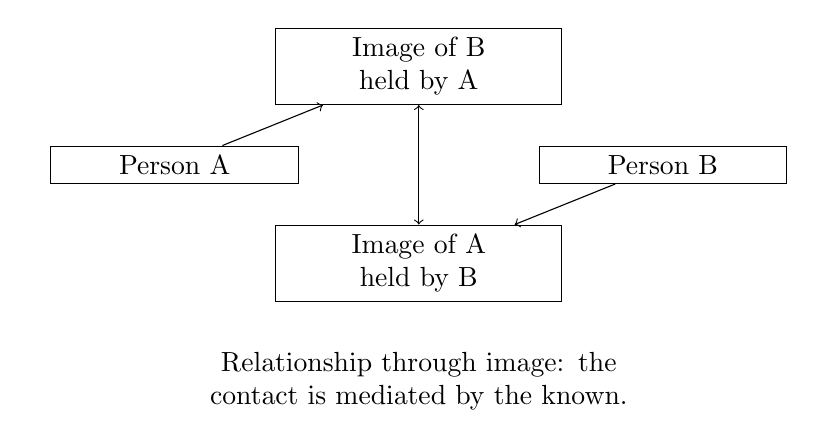
\begin{tikzpicture}
\node[draw, text width=0.24\linewidth, align=center] (a) at (-3.1,0) {Person A};
\node[draw, text width=0.28\linewidth, align=center] (ia) at (0,1.25) {Image of B\\held by A};
\node[draw, text width=0.28\linewidth, align=center] (ib) at (0,-1.25) {Image of A\\held by B};
\node[draw, text width=0.24\linewidth, align=center] (b) at (3.1,0) {Person B};
\draw[->] (a) -- (ia);
\draw[->] (b) -- (ib);
\draw[<->] (ia) -- (ib);
\node[text width=0.80\linewidth, align=center] at (0,-2.75) {Relationship through image: the contact is mediated by the known.};
\end{tikzpicture}
\caption{Relationship through image, reconstructed from the transcript.}
\end{figure}

The direct case is not another theory. It is the negation of the mediating image.

\begin{figure}
\centering
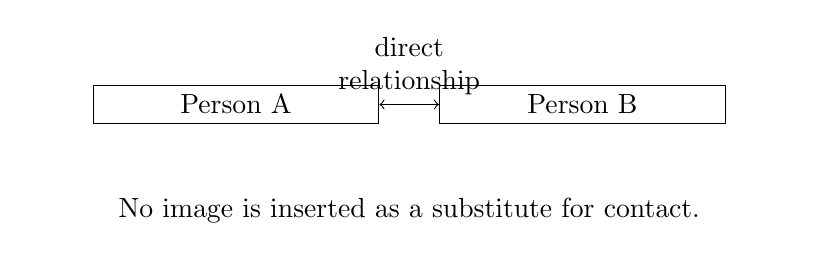
\begin{tikzpicture}
\node[draw, text width=0.28\linewidth, align=center] (a) at (-2.2,0) {Person A};
\node[draw, text width=0.28\linewidth, align=center] (b) at (2.2,0) {Person B};
\draw[<->] (a) -- node[above, align=center] {direct\\relationship} (b);
\node[text width=0.78\linewidth, align=center] at (0,-1.35) {No image is inserted as a substitute for contact.};
\end{tikzpicture}
\caption{A simplified contrast: relationship without image.}
\end{figure}

Anderson's Keats reference enters as a bridge to the present not being betrayed. Krishnamurti does not let the discussion become literary commentary. He brings it back to the fact of relationship. Where there is responsibility in relationship, there is freedom from the known, and the known here is image. In that freedom, he says, goodness flowers. Beauty is not treated as an abstraction; it goes with goodness in behavior, conduct, and action.

\begin{equation}
\text{care}
\longrightarrow
\text{no image in relationship}.
\end{equation}

The movement is cumulative. Responsibility is no longer merely the ground of action. It is now being tested in contact with another human being.

\section{The Fact And The Escape Into Abstraction}

A small verbal correction becomes the central analytic hinge of the lecture. Anderson notices that he often begins with ``if.'' Krishnamurti corrects the movement: not if, but when. The word ``if'' marks a familiar escape. Instead of meeting what is, the mind creates a construction outside the fact, talks about the construction, becomes clever about it, and postpones action.

The example is violence. Krishnamurti begins with the fact: human beings are violent. Because the mind does not know what to do with this fact, it invents the ideal of nonviolence. That ideal is an abstraction from the fact, and therefore a non-fact. The mind then tries to live according to the non-fact, while violence continues.

\subsection{Question \& Answer}

\paragraph{Question.}
Why does the mind create an ideal instead of meeting the fact?

\paragraph{Answer.}
Because it cannot deal with the fact, or does not want to deal with it, or is lazy and postpones action. The ideal makes delay respectable. One says, ``I am trying not to be violent,'' and in the meantime violence continues. Abstraction is therefore an escape from fact.

The sequence should be kept in order:

\begin{align}
\text{fact of violence}
&\longrightarrow \text{ideal of nonviolence}
\longrightarrow \text{postponed action}, \\
\text{abstraction of fact}
&= \text{non-fact}, \\
\text{non-fact}
&\longrightarrow \text{conflict}+\text{misery}+\text{confusion}.
\end{align}

\begin{proposition}
In this lecture, an ideal formed as the opposite of a fact does not resolve the fact. It postpones action and becomes a non-fact.
\end{proposition}

\begin{proof}
Krishnamurti's example supplies the argument.
\begin{enumerate}
\item The fact is violence.
\item The mind abstracts an opposite: nonviolence.
\item The opposite is not the fact; it is a construction away from the fact.
\item To live according to the construction is to postpone meeting violence now.
\item During the postponement, violence continues.
\item Therefore the abstraction produces conflict rather than responsible action.
\end{enumerate}
\end{proof}

\begin{figure}
\centering
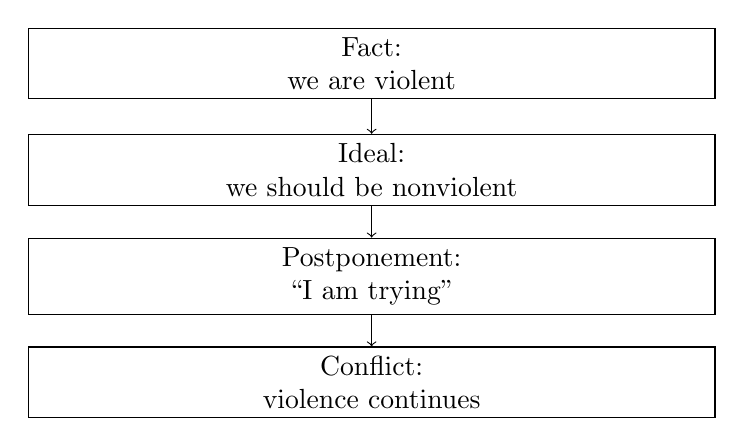
\begin{tikzpicture}
\node[draw, text width=0.70\linewidth, align=center] (f) at (0,0) {Fact:\\we are violent};
\node[draw, text width=0.70\linewidth, align=center] (i) at (0,-1.35) {Ideal:\\we should be nonviolent};
\node[draw, text width=0.70\linewidth, align=center] (p) at (0,-2.7) {Postponement:\\``I am trying''};
\node[draw, text width=0.70\linewidth, align=center] (c) at (0,-4.05) {Conflict:\\violence continues};
\draw[->] (f) -- (i);
\draw[->] (i) -- (p);
\draw[->] (p) -- (c);
\end{tikzpicture}
\caption{The movement from fact to abstraction to conflict. This is a transcript-derived conceptual diagram, not a board reconstruction.}
\end{figure}

Anderson then pauses over the word ``fact.'' Krishnamurti accepts the clarification: call it what is. Fact does not mean merely a recorded item, or ``facts and figures.'' In this inquiry, fact means what is actually present, what is being done. That is why abstraction is so dangerous. It is not only wrong thought; it is withdrawal from the actual.

The same structure returns to relationship. The fact may be that relationship is non-existent because two images are meeting. If the mind escapes into phrases about love, marriage, duty, or values, it again lives on abstraction. The chapter must keep these terms distinct: fact, what is, image, ideal, abstraction, and non-fact are not interchangeable.

\section{Responsibility As Care, Not Prohibition}

The lecture now returns to education and children, but the role of education has changed. Early in the conversation, education tested whether action came from inherited formula. Now it tests care. What is our responsibility for children, not merely one's own children, but children? Are they educated to conform to society, to acquire a job, to continue what has been, to live in abstraction?

Anderson raises the word negation and notes how easily it is mistaken for prohibition. Krishnamurti agrees. Negation is not the command, ``I must not do this, I must not do that.'' It is not will turned negative. It is the direct denial of what is false because the mind sees its implications.

With responsibility go love, care, and attention. Care is not projected into the future as an intention to remember later. It is immediate. It includes affection, consideration, and diligence.

\begin{equation}
\text{freedom}
\longrightarrow
\text{responsibility}+\text{care}+\text{diligence}.
\end{equation}

There is a textual caution. The transcript contains the unstable phrase ``freedom means responsibility and indifference,'' immediately followed by ``infinite care.'' The repeated and coherent movement of the lecture is not toward indifference, but toward care. The chapter therefore preserves the stable relation: freedom, responsibility, care, and diligence belong together.

The opposite of care is not merely cruelty. It can be dependence. Krishnamurti lists dependence on mother, father, teacher, guru, spouse, comfort, and authority. Such dependence trains the child and the adult not to stand alone. When responsibility exists, this structure begins to dissolve. Responsibility for behavior, children, the neighbor, an animal, nature, and the earth makes one astonishingly careful, but not in the sense of obeying prohibitions.

Permissiveness is another false map. Doing what one wants is not freedom.

\begin{equation}
\text{permissiveness}
\not\equiv
\text{freedom}.
\end{equation}

Freedom implies responsibility. Permissiveness breeds irresponsibility. Krishnamurti's anecdote about imported gurus and the child handed over to a religious formation is not a digression. It is a concrete instance of dependence disguised as liberation, and of irresponsibility disguised as spiritual seriousness.

\section{Teacher And Student Learning Together}

Anderson later returns to education from another angle. Suppose there is a school where this responsibility is actually being lived. If the teacher is present to the child, will the child feel it? Krishnamurti accepts the direction, but again makes the question sharper: what is the relationship of teacher and student?

If the teacher is merely an informer, any machine can do that. If the teacher stands above and the student below, division has already entered. But if there is learning on the part of the teacher as well as the student, the division changes. Both are learning. Relationship becomes companionship, sharing, and a journey together.

\begin{align}
\text{teacher as informer}
&\longrightarrow \text{division between teacher and student}, \\
\text{teacher learning}+\text{student learning}
&\longrightarrow \text{companionship}+\text{sharing}.
\end{align}

\begin{figure}
\centering
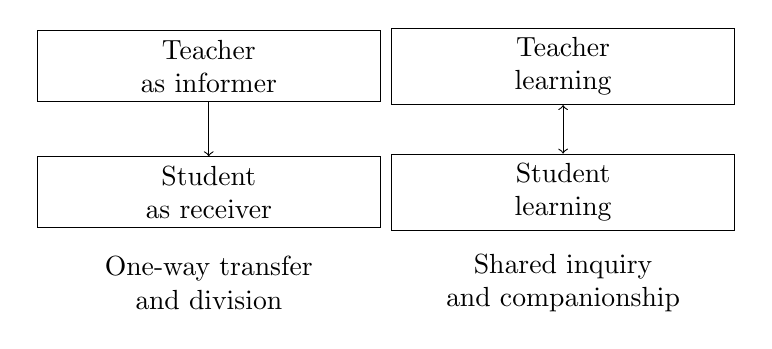
\begin{tikzpicture}
\node[draw, text width=0.34\linewidth, align=center] (t1) at (-2.25,1.2) {Teacher\\as informer};
\node[draw, text width=0.34\linewidth, align=center] (s1) at (-2.25,-0.4) {Student\\as receiver};
\draw[->] (t1) -- (s1);
\node[text width=0.36\linewidth, align=center] at (-2.25,-1.55) {One-way transfer\\and division};

\node[draw, text width=0.34\linewidth, align=center] (t2) at (2.25,1.2) {Teacher\\learning};
\node[draw, text width=0.34\linewidth, align=center] (s2) at (2.25,-0.4) {Student\\learning};
\draw[<->] (t2) -- (s2);
\node[text width=0.36\linewidth, align=center] at (2.25,-1.55) {Shared inquiry\\and companionship};
\end{tikzpicture}
\caption{Two educational structures reconstructed from the teacher-student passage.}
\end{figure}

This is the one place where mathematics is explicitly named. Krishnamurti does not teach a mathematical result. He invokes mathematics as order. The question is how a teacher can teach mathematics so that intelligence is awakened in the child, and how the teaching can convey order in life. Not order according to a blueprint; that, he says, is not order.

\begin{equation}
\text{mathematics}
\longrightarrow
\text{order}.
\end{equation}

Anderson's reference to Simone Weil extends the same point through attention: the subject studied should not be severed from the student's act of attention. The conversation still does not become a formal pedagogy. It remains a question of relationship. Is the teacher training memory like a machine, or helping the student learn about the immensity and complexity of living?

\section{The Responsible Among The Irresponsible}

The final movement asks what a serious person does in a society that trains irresponsibility. Krishnamurti names education, politics, and religion as forces that make human beings irresponsible. Anderson says the work must begin at home, with oneself. Krishnamurti accepts this, but then presses further. What is one's responsibility in the face of the irresponsible?

This passage has to be handled carefully. Krishnamurti speaks tentatively of irresponsible consciousness and responsible consciousness, and of responsibility entering the irresponsible mind in an unconscious way. We should not turn this into a theory of the unconscious. The practical distinction is clearer and sufficient: direct attack produces resistance. The more one actively, designedly operates on another person, the more that person resists and builds a wall.

\begin{align}
\text{designed attack}
&\longrightarrow \text{resistance}, \\
\text{careful pointing out}
&\longrightarrow \text{possible inward seeing}.
\end{align}

The responsible person therefore does not attack, manipulate, or propagandize. Krishnamurti explicitly rejects propaganda. He describes another movement: pointing out what irresponsibility does, showing that it destroys children, sends them to war, and makes them live by books, slogans, and authorities. The medium is care. One cares for the irresponsible person because he is irresponsible, and therefore one watches not to hurt.

At the end, the lecture gathers its strands. Where there is total responsibility, freedom and care go together, and the mind has no image in relationship. Image is division. Where there is care, there is no image.

Anderson sees that this opens toward love and fear. If responsibility and care are continuous, perhaps one could not fear. Krishnamurti agrees that fear must be understood, and also the pursuit of pleasure, because the two go together. But before entering fear, he places one more question before the next conversation: what is order in freedom?

That ending should remain unresolved. This lecture does not answer fear, pleasure, love, or order. It prepares the ground by removing false maps: formula, choice, image, abstraction, prohibition, permissiveness, dependence, and attack.

\section{Summary}

The chapter's logic can be gathered as a sequence of disciplined contrasts. Responsibility for a particular object tends toward direction and will; being responsible is total and undirected. Action from formula continues the past; responsible action is doing now. Choice is not freedom but the sign of confusion; clear seeing acts. Relationship through image is not relationship; image is division. An ideal formed against a fact is abstraction, and abstraction postpones action. Care is not prohibition; it is affection, attention, consideration, and diligence in the present.

The lecture's achievement is not a doctrine of responsibility. It is a clearing away of false responsibility: responsibility to formula, state, guru, image, ideal, permissive self-will, and planned attack. What remains is more exacting: relationship without image, education as shared learning, care that does not wound, and the next unresolved inquiry into order in freedom.